\documentclass[11pt, a4paper]{article}\usepackage[]{graphicx}\usepackage[]{color}
%% maxwidth is the original width if it is less than linewidth
%% otherwise use linewidth (to make sure the graphics do not exceed the margin)
\makeatletter
\def\maxwidth{ %
  \ifdim\Gin@nat@width>\linewidth
    \linewidth
  \else
    \Gin@nat@width
  \fi
}
\makeatother

\definecolor{fgcolor}{rgb}{0.345, 0.345, 0.345}
\newcommand{\hlnum}[1]{\textcolor[rgb]{0.686,0.059,0.569}{#1}}%
\newcommand{\hlstr}[1]{\textcolor[rgb]{0.192,0.494,0.8}{#1}}%
\newcommand{\hlcom}[1]{\textcolor[rgb]{0.678,0.584,0.686}{\textit{#1}}}%
\newcommand{\hlopt}[1]{\textcolor[rgb]{0,0,0}{#1}}%
\newcommand{\hlstd}[1]{\textcolor[rgb]{0.345,0.345,0.345}{#1}}%
\newcommand{\hlkwa}[1]{\textcolor[rgb]{0.161,0.373,0.58}{\textbf{#1}}}%
\newcommand{\hlkwb}[1]{\textcolor[rgb]{0.69,0.353,0.396}{#1}}%
\newcommand{\hlkwc}[1]{\textcolor[rgb]{0.333,0.667,0.333}{#1}}%
\newcommand{\hlkwd}[1]{\textcolor[rgb]{0.737,0.353,0.396}{\textbf{#1}}}%
\let\hlipl\hlkwb

\usepackage{framed}
\makeatletter
\newenvironment{kframe}{%
 \def\at@end@of@kframe{}%
 \ifinner\ifhmode%
  \def\at@end@of@kframe{\end{minipage}}%
  \begin{minipage}{\columnwidth}%
 \fi\fi%
 \def\FrameCommand##1{\hskip\@totalleftmargin \hskip-\fboxsep
 \colorbox{shadecolor}{##1}\hskip-\fboxsep
     % There is no \\@totalrightmargin, so:
     \hskip-\linewidth \hskip-\@totalleftmargin \hskip\columnwidth}%
 \MakeFramed {\advance\hsize-\width
   \@totalleftmargin\z@ \linewidth\hsize
   \@setminipage}}%
 {\par\unskip\endMakeFramed%
 \at@end@of@kframe}
\makeatother

\definecolor{shadecolor}{rgb}{.97, .97, .97}
\definecolor{messagecolor}{rgb}{0, 0, 0}
\definecolor{warningcolor}{rgb}{1, 0, 1}
\definecolor{errorcolor}{rgb}{1, 0, 0}
\newenvironment{knitrout}{}{} % an empty environment to be redefined in TeX

\usepackage{alltt}
\usepackage[margin=1in]{geometry}
\usepackage[utf8]{inputenc}
\usepackage[english]{babel}
\usepackage{csquotes}
\usepackage{longtable, booktabs, tabularx, threeparttable, adjustbox}
\usepackage{amsmath, amssymb, amsthm, bbm, bm}
\usepackage{secdot, sectsty}
\usepackage{hyperref}
\usepackage{pdflscape}
\usepackage{geometry}
\usepackage{placeins}
\usepackage{caption}
\usepackage{graphicx}
\usepackage{setspace}

\usepackage[backend=bibtex, style=authortitle, citestyle=authoryear-icomp, url=false]{biblatex}
\addbibresource{UBIF.bib}

\AtBeginEnvironment{quote}{\singlespacing\small}

\allsectionsfont{\rmfamily}
\sectionfont{\normalsize}
\subsectionfont{\normalfont\normalsize\selectfont\itshape}
\subsubsectionfont{\normalfont\normalsize\selectfont\itshape}

\newcommand{\specialcell}[2][c]{%
      \begin{tabular}[#1]{@{}c@{}}#2\end{tabular}}
\IfFileExists{upquote.sty}{\usepackage{upquote}}{}
\begin{document}
%\SweaveOpts{concordance=TRUE}
%%%This was causing an error for me--not sure why...%

\title{More Than Money: Effects of Cash Transfer Narratives on Agency and Self-Investment}
\begin{onehalfspace}

\author{
  Justin Abraham \thanks{University of California, San Diego.$^{\dagger\dagger}$Contributed
equally.}~$^{\ddagger\ddagger}$,
  Nicholas Otis\thanks{University of California, Berkeley. $^{\dagger\dagger}$Contributed
equally.}~$^{^{\ddagger\ddagger}}$,
  Catherine Thomas\thanks{Stanford University. $^{\dagger\dagger}$Contributed equally.}~$^{^{\ddagger\ddagger}}$,
  Hazel Markus \thanks{Stanford University.},
  Greg Walton \thanks{Stanford University.}
        }

\end{onehalfspace}

\maketitle

\begin{abstract}

    This document describes the pre-analysis plan for a randomized experiment examining the effects of narratives accompanying unconditional cash transfers on self-concept and economic behavior. We provided small, unconditional cash transfers to residents of two informal settlements in Nairobi and randomly assign participants to receive one of three messages with a constant amount of cash. Respondents will receive a message stating that the cash is intended for 1) poverty alleviation, 2) individual empowerment, or 3) community empowerment. We then collected self-reported measures of self-efficacy, stigma, and affect and behavioral measures of future-orientation, self-investment, and program support. This pre-analysis plan outlines our hypotheses, the schedule of experimental tasks, and our empirical strategy. In order to guarantee transparency and bind ourselves from fishing for results, we will pre-register the scripts to be used for data analysis.

\end{abstract}

\newpage

\tableofcontents

\newpage

\section{Introduction}

\section{Research Design}

    \subsection{Sampling}

        This study was conducted in conjunction with the Busara Center for Behavioral Economics (Busara) in Nairobi with 565 participants residing in Kibera and Kawangware, two of Kenya's largest informal settlements \parencite{haushofer_methodology_2014}. Treatment and data collection were conducted by Busara Center enumerators with participants from Kibera and Kawangware in lab and field settings, using tablets to display audio and video media and record participant responses. This section outlines the sampling procedure used in the experiment. \\

        Participants were recruited from the Busara participant pool and were asked to participate in the survey in one of the lab settings. There were seven survey locations used throughout the study period. Table \ref{tab:location} summarizes these areas.

        \begin{table}[h]
        \centering
        \caption{Survey locations}
        \label{tab:location}
        \maxsizebox*{\textwidth}{\textheight}{
        \begin{tabular}{@{}lllll@{}}
        \toprule
        Area & Survey location &  &  &  \\ \midrule
        Kibera & AIC Church &  &  &  \\
        Kibera & Kibera Immanuel Technical Institute &  &  &  \\
        Kibera & Kibera Labour Hall &  &  &  \\
        Kibera & Kibera Chonesus Hall &  &  &  \\
        Kibera & Busara Center (Lab) &  &  &  \\
        Kawangware & Kawangware Pastor Ken's Hall &  &  &  \\
        Kawangware & Kawangware CDF Hall &  &  &  \\ \bottomrule
        \end{tabular} }
        \end{table}

        Participants were recruited to participate in the study if they met the following eligibility criteria:

        \begin{enumerate}
        \itemsep0em
            \item Member of the Busara Center's participant pool
            \item Resident of Kibera or Kawangware
            \item Owns a working phone and an M-Pesa account registered under the participant's name
        \end{enumerate}

    \subsection{Statistical power}

        To achieve power of 80\% for an estimated effect size of 0.30 SD, the required sample size of each arm is 175 participants.

    \subsection{Experimental procedure}

        The survey questionnaire was delivered by enumerators to participants in Swahili or English, as preferred by the participant. The following summarizes the schedule of tasks in the questionnaire.\footnote{We will use a single survey instrument, programmed with Qualtrics, for treatment delivery and subsequent data collection.}

        \begin{enumerate}
        \itemsep0em
            \item Consent agreement
            \item Cash transfer and message (randomized)
            \item Self-efficacy module
            \item Stigma module
            \item Affect module
            \item Video selection task
            \item Savings task
            \item Message evaluation
            \item Support for organization and message
            \item MacArthur Subjective Social Status Ladders (normalized)
            \item Sociodemographic module
        \end{enumerate}

    \subsection{Treatment}

        At the outset of the survey, eligible and consenting participants were told they would be receiving an unconditional cash transfer of KES 400 (USD PPP 10.5) from an organization unaffiliated with the Busara Center.\footnote{This study was conducted with Kenyan shillings (KES). We report USD values calculated at purchasing power parity using a conversion factor for private consumption of 38.15 in 2013. The price level ratio of PPP conversion factor (GDP) to KES market exchange rate for 2011 was 0.444.} \\

        Participants were randomly assigned by the survey software within enumerator\footnote{We evenly assigned treatment groups to achieve balance in group size.} to receive one of three messages introducing the purpose of the cash transfer. The three messages had a similar structure, but we experimentally varied the described purpose of the cash transfer. Specifically, we changed the stated goals of the organization, rationale for providing money, assumptions about recipients, and expectations and goals for the use of the transfer. In the poverty alleviation message, the payment was described as a means to meet basic needs. The individual empowerment message described the payment as a means toward individual goals and advancement. The community empowerment message described the payment as a means toward goals advancing one's family and the community for community advancement. Participants listened to the message twice in their preferred language (English or Swahili) with pre-recorded audio clips or as read by the enumerator. \\

        After hearing the message once, senior enumerators were alerted to use a project MPESA account to send USD PPP 10.5 to the participant via the mobile money system M-Pesa.\footnote{For more information on M-Pesa, we refer the reader to \textcite{jack_mobile_2011} and \textcite{mbiti_mobile_2011}.} Enumerators were instructed to confirm receipt of the payment on the respondent's phone, after which enumerators played the message a second time.\footnote{For the first day and a half of the survey period (for approximately approximately 100 respondents), we used a system in which the respondent texted a code which enabled the direct transfer of the money to their account. Due to technical difficulties, we were required to change to the above system.} Then, enumerators led the respondent's through a series of questions on how they view the transfer. In particular they are asked questions on their current needs (in the ``poverty alleviation'' arm) or goals (in the ``individual empowerment'' and ``community empowerment'' arms), the name they would assign to these funds (for example ``education fund''), how receipt of these funds would affect their relationship with others, and their perceived goal of the organization. \\

        Below, we list the three treatment messages that respondents received: \\

        \textbf{Poverty alleviation message:} \textit{The goal of this Poverty Alleviation Organization is to alleviate poverty and reduce financial hardship among the poor. This organization believes that people living in poverty should be given income support to help them meet their basic needs. This organization aims to help promote a decent standard of living among the poor and help them deal with emergencies. Thus, the Poverty Alleviation Organization gives financial assistance to people like you, to help them make ends meet. For example, with the financial assistance, people might be able to struggle less to afford basic needs, like paying off debts, paying rent, and buying clothes and food. Now we are going to send you 400 KSh. Please note that this is a one-time transfer of financial assistance.} \\

        \textbf{Individual empowerment message:} \textit{The goal of this Individual Empowerment Organization is to promote individuals' potential to create a better future for themselves.  The organization believes that individuals are wise and know best how to help themselves become self-reliant/independent if they have the financial resources to do so. This organization aims to empower individuals to pursue their personal interests and create their own path to independence. Thus, the Individual Empowerment Organization gives financial resources to individuals, like you, to enable them to invest in their personal goals. For example, people might use their unique talents to start a self-run business, invest in job training courses, or create art. Now we are going to send you 400 KSh. Please note that this is a one-time transfer of financial resources.} \\

        \textbf{Community empowerment message:} \textit{The goal of this Community Empowerment Organization is to enable people to help promote better futures for those they care about and want to support most. The organization believes that people know best how to support each other and grow together if they have financial resources to do so. This organization aims to empower people to improve their own lives and those of the people and communities they care about most. Thus, the Community Empowerment Organization gives financial resources to community members, like you, to enable them to contribute positively to the lives of people important to them. For example, when people can invest in themselves, they are better able to expand employment opportunities for others, provide valuable services to their community, or teach others, including children, useful skills and knowledge. Now Community Empowerment Organization is going to send you 400 KSh. Please note that this is a one-time transfer of financial resources.} \\

\section{Data}

    This section describes the data collected following the cash transfer and messaging.

    \subsection{Self-efficacy module}

        This module assesses the extent to which respondents feel capable of improving their lives and the lives of others important to them in the current moment.

        \begin{itemize}
        \itemsep0em
            \item In this moment, how much do you feel in control of your financial situation, such as your success in your business or employment, or other income generating activities.
            \item In this moment, how much do you feel capable of making progress towards your goals.
            \item In this moment, how much do you feel capable of making progress towards goals for your community, such as helping and empowering others you care about.
            \item In this moment, how much do you feel that life will get better?
        \end{itemize}

    \subsection{Stigma module}

        This module assesses the ways in which respondents feel that they or other recipients feel judged by others.

        \begin{itemize}
        \itemsep0em
            \item People may negatively judge others for various reasons. How much do you feel that other people in Kenya make judgments about you based on your economic status? By economic status, I mean things like the place where you live, your job, or the amount of money you have.
            \item How much would other people feel embarrassed if they received money from the [ORGANIZATION NAME]?
            \item If your neighors found out that you received money from the [ORGANIZATION NAME], how upset or jealous would they be with you?
            \item In this moment, how much do you feel like a good family member, whatever that means to you?
            \item In this moment, how much do you feel like a good community member, whatever you means to you?
      \end{itemize}

    \subsection{Affect module}

        The affect module assesses the extent of experienced positive and negative emotional states.

        \begin{itemize}
        \itemsep0em
            \item Recall that you just received some cash from [ORGANIZATION], which has a goal of [ORGANIZATION].
            \item Different experiences and conversations can make people feel different emotions, sometimes sad, sometimes excited, sometimes nervous. We want to know how you're feeling right now, from the time we started this conversation. Please answer as quickly and honestly as you can because we want to get your immediate thoughts.
            \item In this moment, how bad or good do you feel?
            \item In this moment, how embarrassed do you feel?
            \item In this moment, how empowered do you feel?
            \item In this moment, how much do you feel worried/concerned about your finances?
        \end{itemize}

    \subsection{Video selection task}

        This task asked participants to make a choice about watching 3-4 minute video clips. Enumerators described the following six videos and the participant chose to watch two at the end of the survey. Participant could not select the same clip more than once. Video clips were played after the completion of the sociodemographic questionnaire.

        \begin{itemize}
        \itemsep0em
            \item A video from the Mark Angel comedy group, featuring Emanuela (leisure)
            \item A trailer for the Nigerian movie, featuring Ramsey Noah (leisure)
            \item A Noa Ubongo video on math skills for business or CBO management (self-investment)
            \item A video of football highlights from around the world (leisure)
            \item A Noa Ubongo video on using equity and debt for financing business development (self-investment)
            \item A Naswa prank skit (leisure)
        \end{itemize}

        This task provided information on participants' willingness to engage in self-investment (i.e. skills building) activities over leisurely activities. We collected data on the participant's ordered first and second choices. We classified each clip as either for leisure or for self-investment and observe the number of self-investment videos (0, 1, or 2) the participant chooses to watch.

    \subsection{Savings decision task}

        This task allowed participants to invest a portion (either one-quarter or one-half of their initial endowment) in savings with an interest rate of 50\%, to be paid out in two weeks. Enumerators reminded the participant about receiving KES 400 and present the participant with the following two choices.

        \begin{enumerate}
        \itemsep0em
            \item ``If you send us 100 right now, after two weeks you will get back 150 KSh.''
            \item ``If you send us 200 right now, after two weeks you will get back 300 KSh.''
        \end{enumerate}

        If the participant chose to save, enumerators instruct them to send the appropriate amount of money to a project phone number a project phone number using M-Pesa. We also use M-Pesa to complete transfers scheduled in two weeks. To further reduce uncertainty regarding the delayed payment, we provided a phone number for participants to call to follow up on the transaction.

        In addition to observing the participants' intertemporal allocation, we employed the framework of \textcite{johnson_aspects_2007} and elicited thoughts the participant may have regarding the choice to delay payment. This was done prior to the participant making the choice to delay payment. Enumerators asked participants to list up to five `queries' regarding the decision. They were then asked to classify each query as either in favor of or against choosing to save the money. We collected data on both the content of the queries and their classification. We calculated for each participant a standardized median rank difference of aspect types to summarize the tendency to produce delay-favored queries before opposed queries.

        \begin{equation}
            \frac{2 (MR_p - MR_i)}{n}
        \end{equation}

        $MR_p$ is the median rank of queries supporting delayed payment, $MR_i$ is the median rank against delayed payment, and $n$ is the total number of queries listed.

    \subsection{Support for organization and message}

        Participants were reminded of the organization's goal by listening to the audio message treatment once more. They were then asked to evaluate the message and were asked whether they would want to show their support for the organization by recording the organization's message themselves.

        \begin{enumerate}
        \itemsep0em
            \item  How empowering is this recorded message?
            \item  Overall do you like or dislike this audio message?
            \item  This [ORGANIZATION] is asking recipients whether they want to help promote their goal of [ORGANIZATION] by recording the voices of recipients saying their message. They want to share these recordings with possible future recipients as a show of support from current recipients. If you support their goal, you could stay after the survey ends to record the message you heard earlier. Would you like to end after watching the videos, or to continue and do a recording to show support for this organization?
        \end{enumerate}

    \subsection{Messages evaluation}

        We ask participants to forecast how many business videos other participants in different treatment arms would watch. Respondents make forecasts for each treatment arm, starting with the treatment message they received, and tell us their level of confidence, allowing us to roughly calculate how well participants are able to forecast treatment effects, and how these forecasts vary by participant confidence.

    \subsection{Sociodemographic questionnaire (9 items)}

        The final portion of the survey asked participants to report various sociodemographic characteristics including:

        \begin{enumerate}
        \itemsep0em
            \item Participant is female
            \item Participant completed standard 8
            \item Participant is Christian
            \item Age
            \item Participant employment status
            \item Average monthly income (in KSh, log transformed, and Winsorized at the top 1\%)
            \item Consumption in the last seven days (in KSH, log transformed, and Winsorized at the top 1\%)
            \item Participant has KSh 1000 stored away
            \item Difficulty in raising KSh 3000 within 2 days (normalized)
        \end{enumerate}

\section{Empirical Analysis}

    \subsection{Randomization balance checks}

        Although the randomization of the treatment ensures balance across groups in expectation, we test for differences in sociodemographic characteristics using the following specification.

        \begin{equation} \label{eq:balance}
        Y_{i} = \beta_{0} + \beta_{1}\text{\textsc{Ind}}_{i} + \beta_{2}\text{\textsc{Com}}_{i} + \varepsilon_{i}
        \end{equation}

        $Y_{i}$ refers to the sociodemographic variables listed in Table \ref{tab:controlvars} for individual $i$ measured at the end of the survey. \textsc{Ind}$_{i}$ indicates assignment to the individual empowerment message while \textsc{Com}$_{i}$ indicates assignment to the community empowerment message. The reference category in this model is the poverty alleviation message. We will estimate cluster-robust standard errors at the individual level. \\

        We include any sociodemographic variable for which we reject balance as a control variable when estimating treatment effects.

    \subsection{Treatment effect of cash transfer messages}

        We will use the following reduced-form specification to estimate the treatment effect of different messages.\footnote{We will conduct the data analysis outlined in this section using the R programming language with the scripts included in Appendix \ref{sec:rscripts}.}

  		\begin{equation} \label{eq:teffect}
            Y_{i} = \beta_{0} + \beta_{1}\text{\textsc{Ind}}_{i} + \beta_{2}\text{\textsc{Com}}_{i} + \varepsilon_{i}
		\end{equation}

        $Y_{i}$ refers to the outcome variables for individual $i$ measured after the manipulation. The outcome variables described in Table \ref{tab:depvars} will be the focus of this analysis.

        \begin{table}[h]
        \centering
        \caption{Primary outcome variables}
        \label{tab:depvars}
        \maxsizebox*{\textwidth}{\textheight}{
        \begin{tabular}{@{}lllll@{}}
        \toprule
        Variable & Description &  &  &  \\ \midrule
        Video selection & Number of self-investment videos chosen (0, 1, 2 out of 6)  &  &  &  \\
        Savings choice & Amount saved (0 KSh, 100 KSh, 200 KSh) &  &  &  \\
        Message recording & Dummy variable for decision to record message of support &  &  &  \\
        \bottomrule
        \end{tabular} }
        \end{table}

        \textsc{Ind}$_{i}$ indicates assignment to the individual empowerment message while \textsc{Com}$_{i}$ indicates assignment to the community support message. The reference category in this model is the poverty alleviation message. We will estimate cluster-robust standard errors at the individual level. Table \ref{tab:hypotheses} lists the hypotheses we will test using Equation \ref{eq:teffect}.

        \begin{table}[h]
        \centering
        \caption{Hypothesis tests}
        \label{tab:hypotheses}
        \maxsizebox*{\textwidth}{\textheight}{
        \begin{tabular}{@{}lllll@{}}
        \toprule
        Null hypothesis & Description &  &  &  \\ \midrule
        $H_0: \beta_1 = 0$ & Effect of individual empowerment message relative to poverty alleviation message &  &  &  \\
        $H_0: \beta_2 = 0$ & Effect of community empowerment message relative to poverty alleviation message &  &  &  \\
        $H_0: \beta_1 = \beta_2$ & Effect of community empowerment message relative to individual empowerment message &  &  &  \\ \bottomrule
        \end{tabular} }
        \end{table}

        In addition to our primary outcomes, we estimate the effect of the treatment on self-efficacy, stigma, affect, support of message, MacArthur subjective social status ladders, and standardized mean rank difference of thoughts in favor of and against saving. We will analyze these variables by both looking at individual items and constructing summary indices. Indices of self-efficacy, stigma, and affect will be constructed by taking the sum of the normalized constituent items and standardizing the index by its mean and SD.

    \subsection{Covariate adjustment}

        To improve precision, we will apply covariate adjustment with a vector of baseline indicators $\mathbf{X}_i$. We obtain the covariate-adjusted treatment effect estimate by estimating Equation \ref{eq:teffect} including the demeaned covariate vector $\mathbf{\dot X}_{i} = \mathbf{X}_{i} - \mathbf{\bar X}_{i}$ as an additive term and as an interaction with the treatment indicator.

        \begin{equation} \label{eq:controls}
            Y_{i} = \beta_{0} + \beta_{1}\text{\textsc{Ind}}_{i} + \beta_{2}\text{\textsc{Com}}_{i} + \gamma_{0} \mathbf{\dot X}'_i + \gamma_{1}\text{\textsc{Ind}}_{i} \mathbf{\dot X}'_i + \gamma_{2}\text{\textsc{Com}}_{i} \mathbf{\dot X}'_i + \varepsilon_{i}
        \end{equation}

        The set of indicators partitions our sample so that our estimate for $\beta_j$ remains unbiased for the average treatment effect \parencite{lin_agnostic_2013}. We will estimate cluster-robust standard errors at the individual level. We use this model to test the hypotheses detailed in Table \ref{tab:hypotheses} including the control variables listed in Table \ref{tab:controlvars}. These variables were chosen based on prior expectations about their predictive power in relation to the outcomes. Because these covariates were measured after treatment, we exclude any variables found to be significantly correlated with the treatmet. Equation \ref{eq:teffect} without covariate adjustment remains our preferred specification and report both estimates for robustness.

        \begin{table}[h]
        \centering
        \caption{Control variables for covariate adjustment}
        \label{tab:controlvars}
        \maxsizebox*{\textwidth}{\textheight}{
        \begin{tabular}{@{}lllll@{}}
        \toprule
        Variable & Description &  &  &  \\ \midrule
        Gender & Participant is female &  &  & \\
        Education & Participant completed standard 8 &  &  & \\
        Age & Participant age &  &  & \\
        Unemployed & Participant is unemployed &  &  & \\
        Income & Average monthly income (in KSh, log transformed, and Winsorized at the top 1\%) &  &  & \\
        Consumption & Consumption in the last seven days (in KSH, log transformed, and Winsorized at the top 1\%) &  &  & \\
        Savings & Participant has KSh 1000 stored away &  &  & \\
        \bottomrule
        \end{tabular} }
        \end{table}

    \subsection{Heterogeneous treatment effects}

        We will analyze the extent to which the policy messages produced heterogeneous treatment effects with the following specification.

        \begin{equation}
            Y_{i} = \beta_{0} + \beta_{1}\text{\textsc{Ind}}_{i} + \beta_{2}\text{\textsc{Com}}_{i} + \delta_{0} x_i + \delta_{1}\text{\textsc{Ind}}_{i} x_i + \delta_{2}\text{\textsc{Com}}_{i} x_i + \varepsilon_{i}
        \label{eq:heteffect} \end{equation}

        $x_{i}$ is the binary dimension of heterogeneity. $\delta_{1}$ and $\delta_{2}$ identify the heterogeneous treatment effects of the individual empowerment and community empowerment messages relative to the poverty alleviation message. Testing $\delta_{1} = \delta_{2}$ identifies heterogeneous effects between the former two messages. Standard errors are clustered at the individual level. We estimate this model with the  variables summarized in Table \ref{tab:hetvars}. Because these variables were measured after treatment, we exclude any found to be significantly correlated with treatment.

        \begin{table}[h]
        \centering
        \caption{Dimensions of heterogeneity}
        \label{tab:hetvars}
        \maxsizebox*{\textwidth}{\textheight}{
        \begin{tabular}{@{}lllll@{}}
        \toprule
        Variable & Description &  &  &  \\ \midrule
        Gender & Participant is female  &  &  &  \\
        Savings & Participant has KSh 1000 stored away &  &  &  \\
        Education & Participant completed standard 8 &  &  &  \\
        \bottomrule
        \end{tabular} }
        \end{table}

    \subsection{Randomization inference}

        One potential concern is that inference might be invalidated by finite sample bias in estimates of the standard errors. To address this issue, we will conduct randomization inference to test the Fisherian sharp null hypothesis of no treatment effect for every participant \parencite{fisher_design_1935}.\footnote{Note that this is more restrictive than the null hypothesis of zero average treatment effect we will test in the previous section.} We perform Monte Carlo approximations of the exact $p$-values using 10,000 permutations of the treatment assignment. We will then estimate the treatment effct within each $m^{th}$ permutation and calculate the standard Wald statistics for each of our hypothesis tests. We will compare the Wald statistics from the original sample with the distribution of permuted statistics to produce approximations of the exact $p$-values:

        \begin{equation} \label{eq:exactp}
            \hat{p}_{\beta} =  \frac{1}{10,000}\sum_{m=1}^{10,000} \mathbf{1} \Big [ \mathbf{\hat{\beta'}}_m V(\mathbf{\hat{\beta}}_m)^{-1} \mathbf{\hat{\beta}}_m \geq \mathbf{\hat{\beta'}}_{obs.} V(\mathbf{\hat{\beta}}_{obs.})^{-1} \hat{\beta}_{obs.} \Big ]
        \end{equation}

        Following \textcite{young_channeling_2015}, we will permute the data and calculate the regressions for all outcomes within each draw. We will conduct the permutation test for Equations \ref{eq:teffect}, \ref{eq:controls}, and \ref{eq:heteffect}. While we will highglight analytic $p$-values as primary, we report these bootstrapped $p$-values for robustness.

    \subsection{Multiple testing adjustment}

        Given that our survey instrument included several items related to a single behavior or dimension, we will calculate sharpened $q$-values over outcomes in Table \ref{tab:depvars} and \ref{tab:controlvars} to control the false discovery rate \parencite{benjamini_adaptive_2006}. Rather than specifying a single $q$, we will report the minimum $q$-value at which each hypothesis is rejected \parencite{anderson_multiple_2008}. We will apply this correction over each set of outcomes but separately for each hypothesis test and equation. When estimating Equation \ref{eq:heteffect}, we correct over different dimensions of heterogeneity separately. We will report standard $p$-values and use minimum $q$-values as primary in our analysis. Table \ref{tab:summary} summarizes the specified models and methods of statistical inference.

        % \begin{table}[h]
        % \caption{Summary of models}
        % \label{tab:summary}
        % \centering
        % \begin{tabular}{|c|c|>{\centering}p{3.5cm}|}
        % \hline
        %  & Treatment effect & Heterogeneous effects\tabularnewline
        % \hline
        % Equation \ref{eq:teffect} & Yes{*} & Yes{*}\tabularnewline
        % \hline
        % Equation \ref{eq:controls} & Yes{*} & No\tabularnewline
        % \hline
        % \multicolumn{3}{|>{\raggedright}p{11cm}|}{{*}Inference using robust standard errors, approximations of the exact $p$-value, and $p$-values controlling for the FDR.}\tabularnewline
        % \hline
        % \end{tabular}
        % \end{table}

        \begin{table}[h]
        \centering
        \caption{Summary of models}
        \label{tab:summary}
        \maxsizebox*{\textwidth}{\textheight}{
        \begin{tabular}{@{}lll@{}}
        \toprule
         & Treatment effect & Heterogeneous effects  \\ \midrule
        Equation \ref{eq:teffect} & Yes{*} & Yes{*}   \\
        Equation \ref{eq:teffect} with imblanced covariates & Yes{*} & Yes{*}   \\
        Equation \ref{eq:controls} & Yes{*} & No  \\
        \bottomrule
        \multicolumn{3}{>{\raggedright}p{11cm}}{{*}Inference using robust standard errors, approximations of the exact $p$-value, and $p$-values controlling for the FDR.}
        \end{tabular} }
        \end{table}

\newpage

\printbibliography

\newpage

\appendix

\section{Consent Form}
%
%     \maxsizebox*{\textwidth}{\textheight}{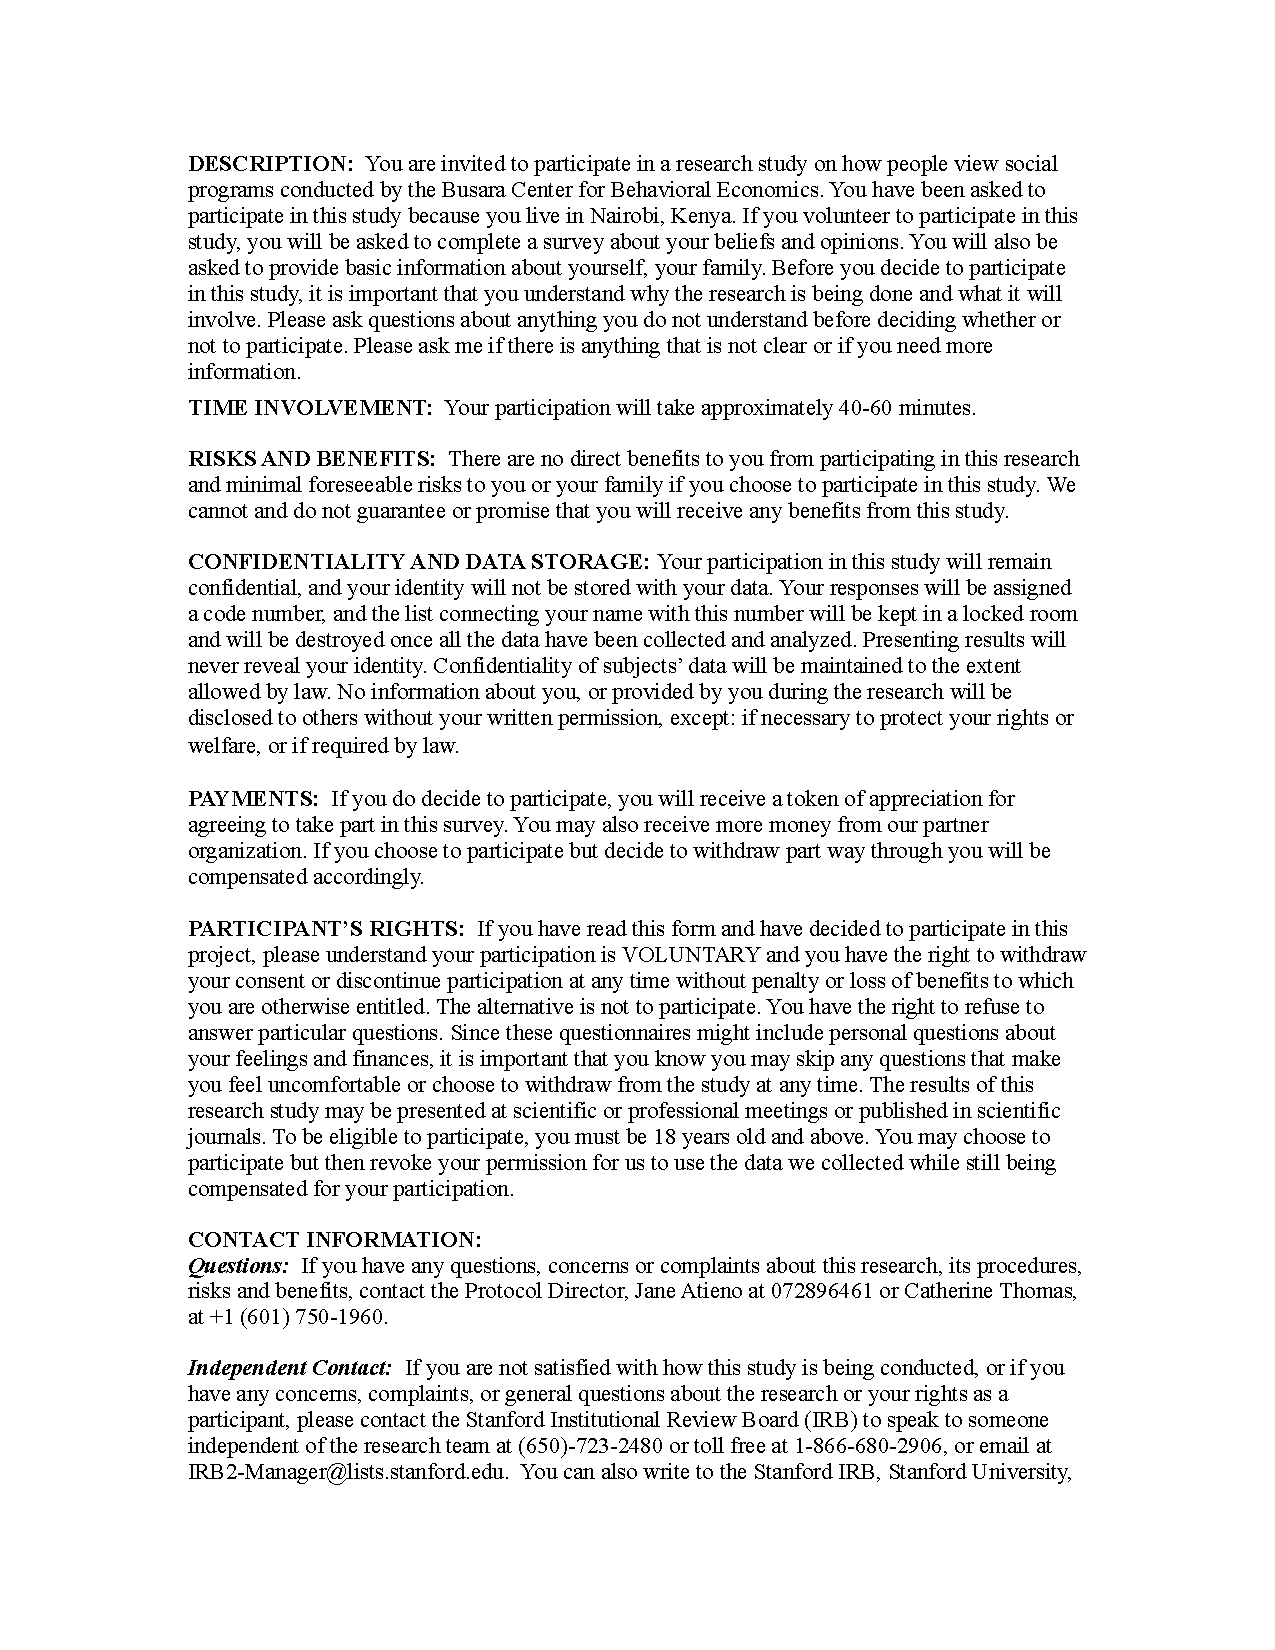
\includegraphics[page=1]{UBI_Consent_S4_Kenya.pdf}}
%     \maxsizebox*{\textwidth}{\textheight}{\includegraphics[page=2]{UBI_Consent_S4_Kenya.pdf}}
%     \maxsizebox*{\textwidth}{\textheight}{\includegraphics[page=3]{UBI_Consent_S4_Kenya.pdf}}
%
% \section{Survey Instrument}
%
\section{Data Analysis Scripts} \label{sec:rscripts}
%
% \begin{footnotesize}
%
% \subsection{Packages}
%
% <<K1packages, results = 'hide', message = FALSE, warning = FALSE>>=
%
%     setwd("/Users/Justin/Google Drive/UBIF/UBIF_Deliverables/UBIF_PAP/K1_PAP")
%     set.seed(47269801)
%
%     required.packages <- c("dplyr", "multiwayvcov", "multcomp", "reshape2", "knitr")
%     packages.missing <- required.packages[!required.packages %in% installed.packages()[,"Package"]]
%
%     if(length(packages.missing) > 0) {install.packages(required.packages, repo="https://cran.cnr.berkeley.edu/")}
%     lapply(required.packages, library, character.only = TRUE)
%
% @
%
%     \subsection{User-defined functions}
%
% <<K1functions, results = 'hide'>>=
%
%     ## RegTest conducts asymptotic test from linear model ##
%
%     RegTest <- function(equation, clustvars, hypotheses, data) {
%
%         model <- lm(equation, data = data, na.action = na.omit)
%
%         if (missing(clustvars)) model$vcov <- vcov(model)
%         else model$vcov <- cluster.vcov(model, cluster = clustvars)
%
%         model$test <- summary(glht(model, linfct = hypotheses, vcov = model$vcov))$test
%
%         numhyp <- length(hypotheses)
%
%         EST <- matrix(nrow = numhyp, ncol = 4)
%
%         for (i in 1:numhyp) {
%
%             EST[i, 1] <- model$test$coefficients[i]
%             EST[i, 2] <- model$test$tstat[i]
%             EST[i, 3] <- model$test$sigma[i]
%             EST[i, 4] <- model$test$pvalues[i]
%
%         }
%
%         colnames(EST) <- c("Estimate", "Tstat", "SE", "P")
%
%         return(EST)
%
%     }
%
%     ## PermTest returns MC approximations of the exact p-value ##
%
%     PermTest <- function(equation, treatvars, clustvars, hypotheses, iterations, data) {
%
%         stopifnot(length(hypotheses) <= 1)
%
%         obsEST <- RegTest(equation, clustvars, hypotheses, data)
%         obsStat <- obsEST[1, 2]
%
%         simEST <- matrix(ncol = 4)
%
%         for (i in 1:iterations) {
%
%             simTreat <- data[, treatvars, drop = FALSE]
%             simTreat <- simTreat[sample(nrow(simTreat)),]
%
%             simData <- cbind(simTreat, data[, !(names(data) %in% treatvars), drop = FALSE])
%             colnames(simData)[1:length(treatvars)] <- treatvars
%
%             simEST <- rbind(simEST, RegTest(equation, clustvars, hypotheses, data = simData))
%
%         }
%
%         simSTAT <- simEST[2:nrow(simEST), 2]
%         countSTAT <- matrix(abs(simSTAT) >= abs(obsStat), ncol = 1)
%
%         ExactP <- colSums(countSTAT) / iterations
%
%         EST <- cbind(obsEST, ExactP)
%
%         colnames(EST) <- c("Estimate", "Tstat", "SE", "P", "ExactP")
%
%         return(EST)
%
%     }
%
%     ## FDR returns minimum q-values ##
%
%     FDR <- function(pvals, step) {
%
%         if (sum(is.na(pvals) == FALSE) <= 1) {return(pvals)}
%         if (missing(step)) {step <- 0.001}
%
%         allpvals <- cbind(as.matrix(pvals), matrix(1:nrow(as.matrix(pvals)), ncol = 1))
%
%         pvals <- na.omit(allpvals)
%         nump <- nrow(pvals)
%
%         pvals <- pvals[order(pvals[, 1]), ]
%         rank <- matrix(1:nump, ncol = 1)
%         pvals <- cbind(pvals, rank, matrix(0, nrow = nump, ncol = 1))
%
%         qval <- 1
%
%         while (qval > 0) {
%
%             qfirst <- qval / (1 + qval)
%             fdrtemp <- (qfirst * rank) / nump
%
%             subrank <- which(fdrtemp >= as.matrix(pvals[, 1]))
%
%             if (length(subrank) < 1) {
%                 numreject <- 0
%             } else numreject <- max(subrank)
%
%             qsec <- qfirst * (nump / (nump - numreject))
%             fdrtemp <- (qsec * rank) / nump
%
%             subrank <- which(fdrtemp >= as.matrix(pvals[, 1]))
%
%             if (length(subrank) < 1) {
%                 numreject <- 0
%             } else numreject <- max(subrank)
%
%             pvals[which(pvals[, 3] <= numreject), 4] <- qval
%
%             qval <- qval - step
%
%         }
%
%         pvals <- pvals[order(pvals[, 2]), ]
%
%         qvals <- matrix(nrow = nrow(allpvals), ncol = 1)
%         qvals[match(pvals[, 2], allpvals[, 2]), 1] <- pvals[, 4]
%
%         return(as.matrix(qvals))
%
%     }
%
% @
%
%     \subsection{Data cleaning}
%
% <<K1data, results = 'hide'>>=
%
%     k1_df <- read.delim(file = "K1__Field_Survey_v34.csv", header = TRUE, sep = ",", stringsAsFactors = TRUE, na.strings = "")
%     k1_df <- as.data.message(k1_df[2:nrow(k1_df), ])
%     attach(k1_df)
%
%     ## Participant ID ##
%
%     k1_df$survey.id <- as.numeric(as.character(k1_df$numb1))
%     k1_df$survey.id[is.na(k1_df$survey.id)] <- as.numeric(as.character(k1_df$numb2))
%     data <- data[complete.cases(k1_df$survey.id), ]
%
%     # sum(duplicated(k1_df$survey.id))
%
%     ## Treatment assignment ##
%
%     k1_df$treatment[k1_df$condition == "poor"] <- 0
%     k1_df$treatment[k1_df$condition == "individual"] <- 1
%     k1_df$treatment[k1_df$condition == "community"] <- 2
%
%     factor(k1_df$treatment)
%
%     k1_df$poor <- ifelse(k1_df$condition == "poor", 1, 0)
%     k1_df$ind <- ifelse(k1_df$condition == "individual", 1, 0)
%     k1_df$com <- ifelse(k1_df$condition == "community", 1, 0)
%
%     k1_df$msg1 <- recode(as.numeric(k1_df$ORG_MESSAGE), `2` = 0, `3` = 2)
%     k1_df$msg2 <- recode(as.numeric(k1_df$ORG_MESSAGE_2), `2` = 0)
%     k1_df$msg3 <- recode(as.numeric(k1_df$ORG_MESSAGE_3), `3` = 2)
%
%     ## Self-efficacy ##
%
%     selvars <- c(k1_df$sel.con, k1_df$sel.pers, k1_df$sel.com, k1_df$sel.prob, k1_df$sel.bett)
%
%     for (var in selvars) {
%
%         var[var == "-99"] <- NA
%
%     }
%
%     k1_df$sel.score <- as.numeric(k1_df$sel.con) + as.numeric(k1_df$sel.pers) + as.numeric(k1_df$sel.com) + as.numeric(k1_df$sel.prob) + as.numeric(k1_df$sel.bett)
%     k1_df$sel.score.z <- (k1_df$sel.score - mean(k1_df$sel.score)) / sd(k1_df$sel.score)
%
%     ## Judgement ##
%
%     judvars <- c(k1_df$jud.fam, k1_df$jud.com, k1_df$jud.judg, k1_df$jud.emb, k1_df$jud.ups)
%
%     for (var in judvars) {
%
%         var[var == "-99"] <- NA
%
%     }
%
%     k1_df$jud.score <- as.numeric(k1_df$jud.fam) + as.numeric(k1_df$jud.com) + (6 - as.numeric(k1_df$jud.judg)) + (6 - as.numeric(k1_df$jud.emb)) + (6 - as.numeric(k1_df$jud.ups))
%     k1_df$jud.score.z <- (k1_df$jud.score - mean(k1_df$jud.score)) / sd(k1_df$jud.score)
%
%     ## Affect ##
%
%     affvars <- c(k1_df$aff.pos, k1_df$aff.ash, k1_df$aff.pow, k1_df$aff.fina)
%
%     for (var in judvars) {
%
%         var[var == "-99"] <- NA
%
%     }
%
%     k1_df$aff.score <- as.numeric(k1_df$aff.pos) + as.numeric(k1_df$aff.pow) + (7 - as.numeric(k1_df$aff.ash)) + (7 - as.numeric(k1_df$aff.fina))
%     k1_df$aff.score.z <- (k1_df$aff.score - mean(k1_df$aff.score)) / sd(k1_df$aff.score)
%
%     ## Video selection ##
%
%     k1_df$vid.imp1 <- ifelse(k1_df$vid.dec1 == "3" | k1_df$vid.dec1 == "5", 1, 0)
%     k1_df$vid.imp2 <- ifelse(k1_df$vid.dec2 == "3" | k1_df$vid.dec2 == "5", 1, 0)
%     k1_df$vid.num <- k1_df$vid.imp1 + k1_df$vid.imp2
%
%     ## Intertemporal choice ##
%
%     k1_df$sav.save = ifelse(k1_df$sav.dec == "2" | k1_df$sav.dec == "3", 1, 0)
%     k1_df$sav.amt[k1_df$sav.dec == "1"] = 0
%     k1_df$sav.amt[k1_df$sav.dec == "2"] = 100
%     k1_df$sav.amt[k1_df$sav.dec == "3"] = 200
%
%     # variable for inconsistent choice, interval estimates of discounting parameter
%     # recode refusals?
%
%     ## Query theory (savings) ##
%
%     que_df <- k1_df[names(k1_df) %in% c("survey.id", "que.rat1", "que.rat2", "que.rat3", "que.rat4", "que.rat5")]
%
%     k1_df$que.nonm <- apply(que_df[, 1:5], 1, function(x) length(x[is.na(x) == FALSE]))
%
%     que_df <- melt(que_df, id = c("survey.id"))
%     que_df$variable <- as.numeric(que_df$variable)
%     que_df$value <- as.numeric(que_df$value)
%     que_df <- dcast(que_df[is.na(que_df$value) == FALSE, ], survey.id ~ value, median, value.var = "variable")
%     names(que_df) <- c("survey.id", "que.mri", "que.mrp")
%     k1_df <- merge(k1_df, que_df, all.x = TRUE)
%
%     k1_df$que.smrd <- (2 * (k1_df$que.mrp - k1_df$que.mri)) / k1_df$que.nonm
%     k1_df$que.smrd[is.na(k1_df$que.mrp)] <- 1
%     k1_df$que.smrd[is.na(k1_df$que.mri)] <- -1
%
%     # dealing with missing by filling in bounds for now, obs with values over this have duplicates
%
%     ## Message evaluation ##
%
%     k1_df$msg.dec <- recode(k1_df$msg.dec, "2" = 1, "1" = 0)
%
%     k1_df$eva.poor[k1_df$msg1 == 0] <- as.numeric(k1_df$eva.msg1[k1_df$msg1 == 0])
%     k1_df$eva.poor[k1_df$msg2 == 0] <- as.numeric(k1_df$eva.msg2[k1_df$msg2 == 0])
%     k1_df$eva.poor[k1_df$msg3 == 0] <- as.numeric(k1_df$eva.msg3[k1_df$msg3 == 0])
%
%     k1_df$eva.ind[k1_df$msg1 == 1] <- as.numeric(k1_df$eva.msg1[k1_df$msg1 == 1])
%     k1_df$eva.ind[k1_df$msg2 == 1] <- as.numeric(k1_df$eva.msg2[k1_df$msg2 == 1])
%     k1_df$eva.ind[k1_df$msg3 == 1] <- as.numeric(k1_df$eva.msg3[k1_df$msg3 == 1])
%
%     k1_df$eva.com[k1_df$msg1 == 2] <- as.numeric(k1_df$eva.msg1[k1_df$msg1 == 2])
%     k1_df$eva.com[k1_df$msg2 == 2] <- as.numeric(k1_df$eva.msg2[k1_df$msg2 == 2])
%     k1_df$eva.com[k1_df$msg3 == 2] <- as.numeric(k1_df$eva.msg3[k1_df$msg3 == 2])
%
%     k1_df$eva.vid.poor <- as.numeric(k1_df$eva.rank.vid_8)
%     k1_df$eva.vid.ind <- as.numeric(k1_df$eva.rank.vid_9)
%     k1_df$eva.vid.com <- as.numeric(k1_df$eva.rank.vid_10)
%
%     k1_df$eva.conf <- as.numeric(k1_df$eva.conf)
%
%     k1_df$eva.emp.poor <- as.numeric(k1_df$eva.rank.emp_5)
%     k1_df$eva.emp.ind <- as.numeric(k1_df$eva.rank.emp_6)
%     k1_df$eva.emp.com <- as.numeric(k1_df$eva.rank.emp_7)
%
%     ## Ladder scales ##
%
%     k1_df$ses.lad.now <- as.numeric(k1_df$ses.lad.now)
%     k1_df$ses.lad.y2 <- as.numeric(k1_df$ses.lad.y2)
%
%     ## Sociodemographics ##
%
%     k1_df$soc.age <- as.numeric(as.character(k1_df$soc.age))
%     k1_df$soc.pri[is.na(k1_df$soc.edu) == FALSE] <- ifelse(as.numeric(k1_df$soc.edu[is.na(k1_df$soc.edu) == FALSE]) >= 4, 1, 0)
%     k1_df$soc.fem[is.na(k1_df$soc.gen) == FALSE] <- ifelse(k1_df$soc.gen[is.na(k1_df$soc.gen) == FALSE] == "2", 1, 0)
%     k1_df$soc.chr[is.na(k1_df$soc.rel) == FALSE] <- ifelse(k1_df$soc.rel[is.na(k1_df$soc.rel) == FALSE] == "1", 1, 0)
%     k1_df$ses.unemp <- ifelse(k1_df$ses.emp == "1", 1, 0)
%     k1_df$soc.inc <- as.numeric(k1_df$soc.inc)
%     k1_df$soc.con <- as.numeric(k1_df$soc.con)
%     k1_df$soc.sav <- as.numeric(k1_df$soc.sav) - 1
%
%     ## Survey validity ##
%
%     k1_df$end.hear <- as.numeric(k1_df$end.hear) - 1
%
% @
%
%     \subsection{Treatment effect}
%
% <<K1teffects, results = 'hold'>>=
%
%     hypotheses <- c("ind = 0", "com = 1", "ind - com = 0")
%     depvars <- c("vid.num", "sav.save", "msg.dec")
%     mechvars <- c("sel.score", "jud.score", "aff.score", "que.smrd", "ses.lad.now", "ses.lad.y2")
%
%     for (h in hypotheses) {
%
%         RES <- matrix(nrow = 1, ncol = 5)
%
%         for (depvar in depvars) {
%
%             eqn <- paste(depvar, "~ ind  + com", sep = " ")
%             RES <- rbind(RES, PermTest(eqn, treatvars = c("treatment", "poor", "ind", "com"), clustvars = k1_df$survey.id, hypotheses = c(h), iterations = 100, data = k1_df))
%
%         }
%
%         RES <- RES[2:nrow(RES), 1:ncol(RES)]
%         RES <- cbind(RES, FDR(RES[, 4]))
%
%         rownames(RES) <- depvars
%         colnames(RES)[6] <- "Min. Q"
%
%         print("----------------------------------------------------------------", quote = FALSE)
%         print(paste("H_0:", h), quote = FALSE)
%         print(RES, quote = FALSE)
%
%     }
%
%     for (h in hypotheses) {
%
%         RES <- matrix(nrow = 1, ncol = 5)
%
%         for (depvar in mechvars) {
%
%             eqn <- paste(depvar, "~ ind  + com", sep = " ")
%             RES <- rbind(RES, PermTest(eqn, treatvars = c("treatment", "poor", "ind", "com"), clustvars = k1_df$survey.id, hypotheses = c(h), iterations = 100, data = k1_df))
%
%         }
%
%         RES <- RES[2:nrow(RES), 1:ncol(RES)]
%         RES <- cbind(RES, FDR(RES[, 4]))
%
%         rownames(RES) <- mechvars
%         colnames(RES)[6] <- "Min. Q"
%
%         print("----------------------------------------------------------------", quote = FALSE)
%         print(paste("H_0:", h), quote = FALSE)
%         print(RES, quote = FALSE)
%
%     }
%
% @
%
%     \subsection{Covariate-adjustment}
%
% <<K1covadj, results = 'hold'>>=
%
%     covariates <- c("soc.fem", "soc.age", "soc.pri", "soc.chr", "soc.sav", "ses.unemp", "soc.inc")
%
%     for (h in hypotheses) {
%
%         RES <- matrix(nrow = 1, ncol = 5)
%
%         for (depvar in depvars) {
%
%             eqn <- paste(depvar, "~ ind  + com +", covariates, sep = " ")
%             RES <- rbind(RES, PermTest(eqn, treatvars = c("treatment", "poor", "ind", "com"), clustvars = k1_df$survey.id, hypotheses = c(h), iterations = 100, data = k1_df))
%
%         }
%
%         RES <- RES[2:nrow(RES), 1:ncol(RES)]
%         RES <- cbind(RES, FDR(RES[, 4]))
%
%         rownames(RES) <- depvars
%         colnames(RES)[6] <- "Min. Q"
%
%         print("----------------------------------------------------------------", quote = FALSE)
%         print(paste("H_0:", h), quote = FALSE)
%         print(RES, quote = FALSE)
%
%     }
%
% @
%
%     \subsection{Heterogeneous treatment effects}
%
% <<K1het, results = 'hold'>>=
%
%     hetvars <- c("soc.fem", "soc.age", "soc.pri", "soc.chr", "soc.sav", "ses.unemp")
%
%     for (hetvar in hetvars) {
%
%         hypotheses <- c(paste("ind:", hetvar, " = 0", sep = ""), paste(hetvar, ":com", " = 0", sep = ""), paste("ind:", hetvar, " - ", hetvar, ":com", " = 0", sep = ""))
%
%         for (h in hypotheses) {
%
%             RES <- matrix(nrow = 1, ncol = 5)
%
%             for (depvar in depvars) {
%
%                 eqn <- paste(depvar, " ~ ind*", hetvar, " + com*", hetvar)
%                 RES <- rbind(RES, PermTest(eqn, treatvars = c("treatment", "poor", "ind", "com"), clustvars = k1_df$survey.id, hypotheses = c(h), iterations = 100, data = k1_df))
%
%             }
%
%             RES <- RES[2:nrow(RES), 1:ncol(RES)]
%             RES <- cbind(RES, FDR(RES[, 4]))
%
%             rownames(RES) <- depvars
%             colnames(RES)[6] <- "Min. Q"
%
%             print("----------------------------------------------------------------", quote = FALSE)
%             print(paste("H_0:", h), quote = FALSE)
%             print(RES, quote = FALSE)
%
%         }
%
%     }
%
% @
%
% \end{footnotesize}

\end{document}
